
\chapter{Chapter3 Performance}

Models suitable for real-life deployment should be not only fast but also accurate. Definitonon of "accurate" differs in literature. In this paper we use top1 classification accuracy on imagenet as proxy for model performance on down-stream tasks, see \ref{subsec: imagenet} for detailed discussion. 
The performance of a vision model is a product of the architecture, training methods and regularization. \cite{lee2020_compounding_improvements}. 
Since the introduction of AlexNet \cite{krizhevsky2012_imagenet_alexnet}, many stuides emphasizes was on modifing model architectures through new blocks (cite Inception), new architectural choices (cite ResNet ), new rules for scaling models \cite{tan2019_efficientnet} or novel types of regularization. \cite{zhang2017_mixup} \cite{yun2019_cutmix}
% тут можно ещё подробнее написать кто что предлагает
In contrast to these studies focusing on designing new network architecture, works like \cite{he2019bag_of_tricks} follow different approach to improve model performance. They noted that performance can be improved not only through changes in the model structure, but also through other aspects of network training such as data preprocessing, augmentations, regularization techniques and parameter initialization (cite NFNet). They also demonstrate that these minor “tricks” play a major part in boosting model performance when applied in combination. This improvements are highly significant because it could bring as much performance improvement as a novel network design does. For example \cite{he2019bag_of_tricks} shows that top-1 validation accuracy of vanilla ResNet-50 could be improved from 75.3\% to 79.29\% with changes in training procedure alone. 

% As a result of using these tricks, ILSVRC2012 top-1 validation ac- curacy of ResNet-50 improved from 75.3\% to 79.29\% and MobileNet improved from 69.03\% to 71.90\%. This im- provement is highly significant because it shows as much performance improvement as a novel network design does. 

There is another issue, rarely mentioned in papers. Novel architectures quite often are introduced simultaneously with other important, but less emphasized changes in the details of training methodology and hyperparameters, most refinements are either briefly mentioned as implementation details or only visible in source code. Additionally novel architectures obtained with modern training strategies are sometimes compared to older architectures with outdated training methodology. This systematic error makes comparing new architectures confusing and makes it much more difficult for practitioners to select good-performing architectures. 

% выше последнее предложение как-то не очень хорошо написано конечно 

This work carefully explores current CNN-related techniques for image classification which could be assembled together, and separates then into training / regularization techniques and architectural changes. The first one being non-intrusive, model-agnostic changes capable of boosting almost any existing convolutional deep learning model. And the second one being modifications of architecture, which greatly affect performance with minor impact on model throughput. 



\section{Preliminaries}
For better understanding we first describe default experimental setup for training ResNet50 model along with it's architecture and description of used dataset and metrics. 

\subsection{Dataset} \label{subsec: imagenet}

% эту часть нужно перенести в главу 4 про эксперименты
% (сюда можно дописать еще общих слов из \cite{beyer2020_are_we_done}) для объема

Imagenet Large Scale Vision Recognition Challenge also known as ILSVRC2012 or simply Imagenet has been a central testbed of research in artificial perception for almost a decade and it's scale and difficulty have highlighted landmark achievements in machine learning. It has 1.3 millions training images divided into 1000 classes. Validation dataste consist of 50 thousand images, equally balanced between same 1000 classes. ILSVRC2012 is the most used dataset in computer vision. % \cite{something related}
In recent years with models becoming larger and demanding more and more data, it became a de-facto stardart benchmark for any new architecture. Since the breakthrought of AlexNet improving convolutional neural networks lead to improvements in other fields of computer vision. Typically researchers optimize models on classification problems using ImageNet \cite{deng2009_imagenet} as proxy. It has been shown \cite{he2019bag_of_tricks} \cite{kornblith2019_better} than improvments from Imagenet increase transfer learning performance other domains, for example object detection and semantic segmentation.


In this papepr we will use top1 1 classification accuracy on the ILSVRC2012 validation dataset as metric of model performance. It has a very strong correlation of $r=0.96$ \cite{kornblith2019_better} between ImageNet accuracy and transfer accuracy, which makes it a well suitable metric.  

\subsection{Baseline Training Procedure} \label{subsec: baseline_training}
This section introduces training hyperparameters for Imagenet following \cite{he2016identity_resnetv2} paper. The preprocessing differs between training and validation. Steps performed during training:
\begin{itemize}
    \item Sample a random image and decode it into 32-bit floating point raw pixel values in [0, 255].
    \item Randomly crop a rectangular region whose aspect ratio is randomly sampled in [3/4, 4/3] and area randomly sampled in [8\%, 100\%], then resize the cropped region into a 224-by-224 square image.
    \item Flip horizontally with 0.5 probability.
    \item Scale hue, saturation, and brightness with coefficients uniformly drawn from [0.6, 1.4].
    \item Add PCA noise with a coefficient sampled from a normal distribution N (0, 0.1)
    \item Normalize RGB channels by subtracting 123.68, 116.779, 103.939 and dividing by 58.393, 57.12, 57.375, respectively.
\end{itemize}

For validation image's shortest edge is first resized to 256 pixels with aspect ratio remaining the same. Secondly a center 224-by-224 region of the image is cropped and RGB channels are normalized similar to training. No random augmentations are performed during validation. 
% TODO: rewrite this copy-pasted piece below
The weights of both convolutional and fully-connected layers are initialized with the Xavier algorithm [6]. In par- ticular, we set the parameter to random values uniformly drawn from $[−a, a]$, where $ a = \sqrt{6 / (d_{in} + d_{out})} $ Here $d_{in}$ and $d_{out}$ are the input and output channel sizes, respectively. All biases are initialized to 0. For batch normalization layers, $\gamma$ vectors are initialized to 1 and $\beta$ vectors to 0.
Stochastic Gradient Descent (SGD) is used for training. Model is trained for 100 epochs a batch size of 256 per GPU. The learning rate is initialized to 0.1 and divided by 10 at the 30th, 60th, and 90th epochs. % TODO \cite{something for SGD}

% TODO: maybe add more details about drawbacks of current architecture 
This training pipeline was de-facto standard for researchers of Imagenet, despite in several drawbacks discussed later. 

\subsection{Baseline Model Architecture}
This section briefly presents the ResNet architecture, especially its modules. For detailed information please refer to \cite{he2016deep_resnetv1}


\begin{figure}[h!]
    \caption{The architecture of ResNet-50. The convolution kernel size, output channel size and stride size (default is 1) are illustrated, similar for pooling layers}
    \label{fig: resnet-a}
    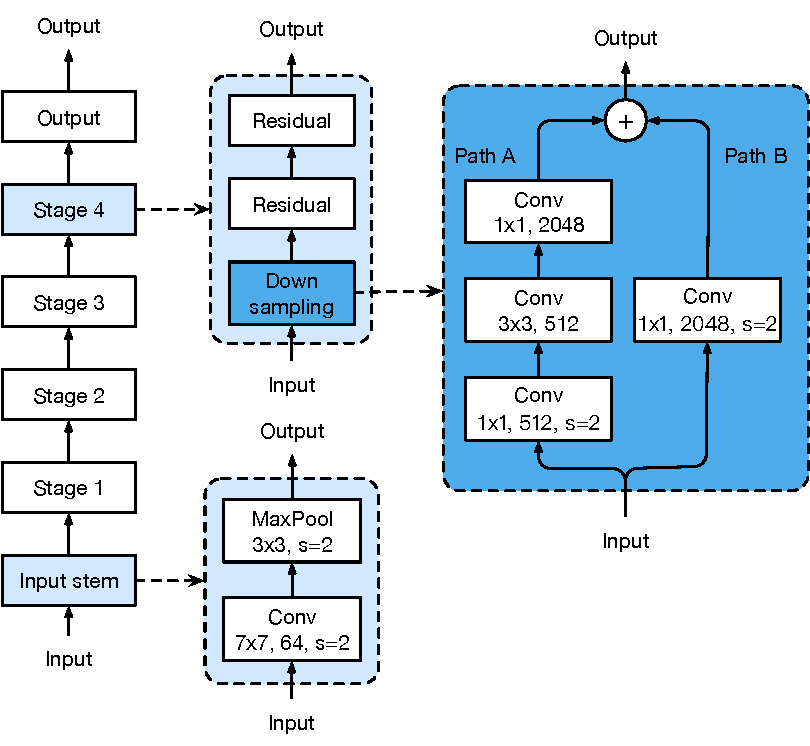
\includegraphics[width=0.5\textwidth]{images/resnet-a.pdf}
  \end{figure}


% below is again a large copy-paste
A ResNet network consists of an input stem, four subsequent stages and a final output layer, which is illustrated in \ref{fig: resnet-a}. The input stem has a $7 \times 7$ convolution with an output channel of 64 and a stride of 2, followed by a $3 \times 3$ max pooling layer also with a stride of 2. The input stem reduces the input width and height by 4 times and increases its channel size to 64. 
Starting from stage 2, each stage begins with a downsampling block, which is then followed by several residual blocks. In the downsampling block, there are path A and path B. Path A has three convolutions, whose kernel sizes are $1 \times 1$, $3 \times 3$ and $1 \times 1$, respectively. The first convolution has a stride of 2 to halve the input width and height, and the last convolution’s output channel is 4 times larger than the previous two, which is called the bottleneck structure. Path B uses a 1×1 convolution with a stride of 2 to transform the input shape to be the output shape of path A, so we can sum outputs of both paths to obtain the output of the downsampling block. A residual block is similar to a downsampling block except for only using convolutions with a stride of 1.
One can vary the number of residual blocks in each stage to obtain different ResNet models, such as ResNet-50 and ResNet-152, where the number presents the number of convolutional layers in the network.


% 
% 2.1. Baseline Training Procedure
% We follow a widely used implementation [8] of ResNet as our baseline. The preprocessing pipelines between train- ing and validation are different. During training, we per- form the following steps one-by-one:
% 1. Randomly sample an image and decode it into 32-bit floating point raw pixel values in [0, 255].
% 2. Randomlycroparectangularregionwhoseaspectratio is randomly sampled in [3/4, 4/3] and area randomly sampled in [8%, 100%], then resize the cropped region into a 224-by-224 square image.
% 3. Flip horizontally with 0.5 probability.
% 4. Scale hue, saturation, and brightness with coefficients
% uniformly drawn from [0.6, 1.4].
% 5. Add PCA noise with a coefficient sampled from a nor-
% mal distribution N (0, 0.1).
% 6. Normalize RGB channels by subtracting 123.68, 116.779, 103.939 and dividing by 58.393, 57.12, 57.375, respectively.
% During validation, we resize each image’s shorter edge to 256 pixels while keeping its aspect ratio. Next, we crop out the 224-by-224 region in the center and normalize RGB channels similar to training. We do not perform any random augmentations during validation.
% The weights of both convolutional and fully-connected layers are initialized with the Xavier algorithm [6]. In par- ticular, we set the parameter to random values uniformly drawn from [−a, a], where a = 􏰇6/(din + dout ). Here din and dout are the input and output channel sizes, respec- tively. All biases are initialized to 0. For batch normaliza- tion layers, γ vectors are initialized to 1 and β vectors to 0.
% Nesterov Accelerated Gradient (NAG) descent [20] is used for training. Each model is trained for 120 epochs on 8 Nvidia V100 GPUs with a total batch size of 256. The learning rate is initialized to 0.1 and divided by 10 at the 30th, 60th, and 90th epochs.


% тут нужно как-то сказать что в этой главе мы меняем только базовый резнет, а более серьзеные изменения, объединяющие выводы главы 2 и 3 представлены в главе 4


\section{Training methods}

Here we present regularization and data augmentation strategies routinely used in state-of-the art classification models \cite{lin2020neural_genet} \cite{tan2019_efficientnet} \cite{tan2021_efficientnetv2}

\subsection{Data Augmentation}
Default augmentations used in Imagenet training described in \ref{subsec: baseline_training} are quite weak to match up the capacity of modern CNNs. Many better augmentations strategies has been proposed to bring diversity during training. Two most popular being: 

\begin{itemize}
    \item AutoAugment \cite{cubuk2018_autoaugment} which learngs augmentation strategies from data. It uses reinforcement learning to select a sequence of image augmentation operations with the best accuracy by searching a discrete search space of their probability of application and magnitude.
    \item RanAug \cite{cubuk2020_randaugment} also applies reinforcement learning, but to a significatly reduced search space in order to find sequence of random image transformations (e.g. translate, shear, color distortions) for each image
\end{itemize}

\begin{figure}[h!]
    \caption{One of the successful policies on ImageNet. As described in the text, most of the policies found on ImageNet used color-based transformations.}
    \label{fig: randaug}
    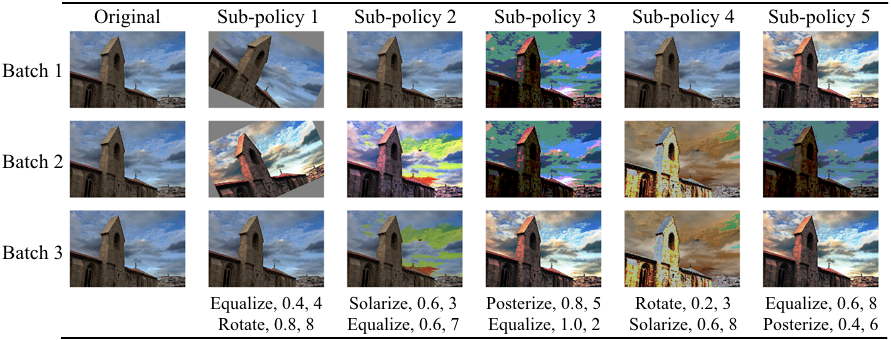
\includegraphics[width=0.5\textwidth]{images/randaug_policy.png}
  \end{figure}

Both of this policies use extensive amount of augmentations in the color domain combined with hard affine transformations like rotation and shear. Example of augmentations could be seen on \ref{fig: randaug}
From out experiments we found that RandAug slightly overperforms AutoAugment, so we use the former later in the text. The exact definition of RandAug augmentation strategy on Imagenet could be found in Appendix. 
% TODO: add RandAug strategy to appendix.


\subsection{MixUp and CutMix}

% TODO: fix this table, remove cutout from it
% original cutmix table. I don't know how to increase it so using the version below for now. But this one looks better IMHO
% \begin{table}[h!]
%   \centering
%   \small
%   \tabcolsep=0.07cm
%   \begin{tabular}{@{}ccccc@{}}
%   & Original  &  Mixup \cite{zhang2017_mixup} & CutMix \cite{yun2019_cutmix}\\
%   \multirow{4}{*}{Image} &  \multirow{4}{*}{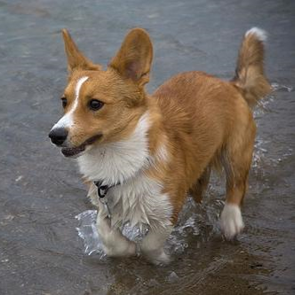
\includegraphics[width=0.10\linewidth]{images/dog.png}}
%   &  \multirow{4}{*}{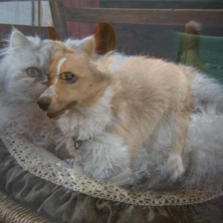
\includegraphics[width=0.10\linewidth]{images/dog_mixup.png}}
%   &  \multirow{4}{*}{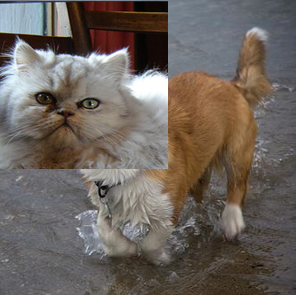
\includegraphics[width=0.10\linewidth]{images/dog_cutmix.png}} \\ 
%   & & & \\ 
%   & & & \\
%   & & & \\ \midrule
%   %
%   \multirow{2}{*}{Label} 
%   &\multirow{2}{*}{Dog 1.0}
%   &\multirow{2}{*}{\begin{tabular}[c]{@{}c@{}}Dog 0.5\\ Cat 0.5\end{tabular}}
%   &\multirow{2}{*}{\begin{tabular}[c]{@{}c@{}}Dog 0.6\\ Cat 0.4\end{tabular}} \\ 
%     & & & \\  \toprule

%   \end{tabular}
%   \caption{Example of Mixup/CutMix augmentations}
%   \label{tab:cutmix}
%   \end{table}


  \begin{figure}[h!]
    \centering
    \subfloat[][Original \\ Dog 1.0]{
      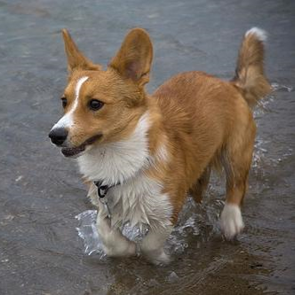
\includegraphics[scale=.55]{images/dog.png}
    }\hfill%
    \subfloat[][Mixup \\ Dog 0.5 Cat 0.5]{
      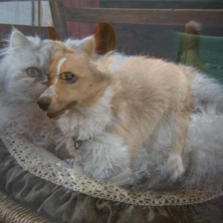
\includegraphics[scale=.55]{images/dog_mixup.png}
    }\hfill%
    \subfloat[][Cutmix \\ Dog 0.6 Cat 0.4]{
      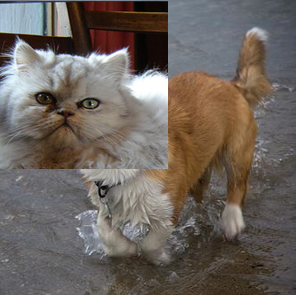
\includegraphics[scale=.55]{images/dog_cutmix.png}
    }
    \caption{Example of Mixup/CutMix augmentations. Label for each image during training is shown in sub-captions.}
    \label{fig:cutmix}

  \end{figure}

Mixup \cite{zhang2017_mixup} and CutMix \cite{yun2019_cutmix} are two recently proposed augmentation and regularization strategies. They both create new examples by interpolating two examples of the training set. Neural networks are known to memorize training data rather than generalize from the data \cite{zhang2016_understanding_deep}. As a result, the neural network produces unexpected outputs when it encounters data which are different from the distribution of the training set. Mixup/CutMix mitigates the problem by showing the neural network interpolated examples, and this helps to fill up the empty feature space of the training dataset.

% below is copy-paste
CutMix shares simularity with Mixup which mixes two samples by interpolating both the image and labels. While certainly improving classification performance, Mixup samples tend to be unnatural and locally ambiguous, and therefore confuses the model. CutMix overcomes the problem by replacing the image region with a patch from another training image, producing a more natural results as could be seen on \ref{tab: cutmix}

Mixup/CutMix has two types of implementation. The first type uses two mini batches to create a mixed mini batch. this type of implementation is suggested in the original paper \cite{zhang2017_mixup}. The second type uses a single mini batch to create the mixed mini batch by mixing the single mini batch with a shuffled clone of itself. The second type of implementation uses less CPU resources because only one mini batch needs to be preprocessed to create one mixed mini batch. However, experiments show that the second type of implementation reduces top-1 accuracy \cite{lee2020_compounding_improvements}. Therefore, in later experiments, we use the first type of implementation. We set the Mixup hyperparameter $\alpha$ to 0.2 and Cutmix alpha to 1. 

% TODO: вставить больше формул про то, что такое CutMix https://sh-tsang.medium.com/paper-cutmix-regularization-strategy-to-train-strong-classifiers-with-localizable-features-5527e29c4890


%% END OF SECTION

% The following section 
% Novel architectures are often simultaneously introduced with other critical – and less publicized – changes in the details of the training methodology and hyperparameters. Additionally, new architec- tures enhanced by modern training methods are sometimes compared to older architectures with dated training meth- ods (e.g. ResNet-50 with ImageNet Top-1 accuracy of 76.5\% \cite{he2016deep_resnetv2}. Our work addresses these issues and empirically studies the impact of training methods and scaling strategies on the popular ResNet architecture





%% 
% уже писал, но можно написать план еще раз. говорю, что новые статьи улучшаются и за счет блоков и за счёт улучшения тренировки, причем часто авторы статей не разделютя одно от другого, хочется посмотреть, на что способны старые архитектуры, если учить их новыми методами (это примерно то что пишут авторы резнет РС). в этой главе бОльшую часть нужно потратить на обзор маленьких улучшений, предложенных в последние годы (???)

%%
% нужно понять в каком порядке излагать мысль вообще. есть статьи, которые улучшают архитектуру, а есть которые предлагают новые способы обучения. проблема в том, что это не всегда разные статьи. новые блоки часто идут вместе с новыми трюками и сложно их разделить. (о чём пишут в compunding performance и гораздо более явно в resnet-RS). можно написать то же самое и скзаать что "я был первым" что на самом деле так, я об этом еще в начале прошлого года расговаривал). но мне для диплома нужно много текста, поэтому надо как-то завернуть рассжудения. как завернуть? 

% разница между compunding и resnetRS в том, что первые бустят resnet без явного разделения что приходит от новых методов, а что приходит от изменения архитектуры, а RS явно показывает что приходит от архитектуры. 

%%





% at- tempts to combine existing techniques to create a practi- cal model are still uncommon

(нужно еще где-то сказать что со временем растет уровень того что такое бейзлайн. если в 2016м году резнет50 был 75.6, то сейчас если он ниже 79, то сравнение нечестное. самое честное что можно (и нужно делать) это использовать одинаковые трюки как во время обучения своей новой супер-пупер мега модели так и во время обучения старого-доброго резнета)



\subsection{How to do better}



(когда буду говорить про пайплайн, нужно вставить что дефолтные аугментации очень слабые и хотя это uncommon to report training accuracy for the model, one can observe a very strong overfitting using the default augmentation. it means that almost any additional regularization would have a noticable effect, but it also means that что они бьют лежачего в общем    )


The questin is, when does ResNet50 stop being ResNet50? How many architecture changes is needed to be able to call it a new model? Why majority of people do not modify block structure, while making strong modifications of blocks themselves? The anwser is probably because experiments on ImageNet are quite expensive and not everyone has resources and time and knowledge to explore all possible variations. This is where papers like mine come into place with thorough examination of already proposed techniques and how do they combain together

% когда буду говорить про переход к ResNet D нужно не просто предсатвить новую архитектуру, а попытаться объяснить какие именно проблемы она решает. типо страйд не там или что

(когда буду говорить про MixUp сделать ремаку о том что есть два типа (внутри батча и с другим батчом) и что второй вариант работает лучше, ссылаясь на свои собственные эксперименты если найде или на Componding). 


(когда буду говорить про SE vs ECA сделать ремарку о том, что авторы второго не правы, когда мерят ФЛОПс и говорят что у них меньше. может быть добавить экспреименты со скоростью если делать просто GAP без каких либо операций и показать что он занимает бОльшую чать от замедления (сколько это кстати? 60? 70?))



% (тут ли?)
% Говорю о том что в последнее время появилось много малненьких улучшений, которые не замедляют сеть, но дают буст по качетсву \cite{zhang2019making_aa_shift_invariant} или space2depth  \cite{ridnik2021_tresnet} в начале сети. были статья которые объединяли это все вместе \cite{lee2020compounding_improvements} \cite{bello2021revisiting_resnet} (ну и как бы мои результаты не лучше чем у них, просто они тупо стакают все изменения на резнет, а я еще и архитектуру меняю после этого, чтобы учесть архитектруные недостатки


% говно разбиение на главы. чем глава 3 отличается от главы 4?
% в 3.1 говорю про улучшения тренирочного пайплайна, в 3.2 про улучшения архитектуры? 
% но нужно как-то подвести к этому, а не тупо начинать вываливать на читатлеей списки новых слоёв??


% Глава2 - про скорость и связь со флопсами и все такое
% Глава3 - про улучшения обучения связанные с ванильным R50
% Глава4 - про связку небольших изменений и медленные изменения архитектуры опираясь на то, что работает у других
% Глава5 - design choice not present in current literature

